% Lines that start with a % are comments and are not included when the LaTeX file is converted to a pdf

% Set up the document class - this can be changed if a different format is required 
\documentclass[11pt,a4paper,twoside]{article}

% Include packages that contain additional features, for example including special mathematical characters and images in your document
\usepackage{amssymb,amsmath,graphicx}
\usepackage[T1]{fontenc} 
\usepackage[utf8]{inputenc}   % here are our umlauts...
\usepackage{graphicx} % ...and our graphics
\usepackage{listings}
\usepackage{bold-extra}
\usepackage[plainpages=false, pdfpagelabels, colorlinks=true, breaklinks=true, linkcolor=black, menucolor=black, urlcolor=black, citecolor=black]{hyperref}
\usepackage[font=sf, labelfont={sf,bf}, margin=1cm]{caption}
\usepackage[b]{esvect}
% Long equations
\usepackage{breqn} 
%include pdfs
\usepackage{pdfpages}
\usepackage{epstopdf}
\usepackage{fullpage}


% The beginning of the document...
\begin{document}
\renewcommand\thesubsection{\alph{subsection})}

% configure standard code listings:
\lstset {
language = bash,
	breaklines = true,
	breakatwhitespace = true
}

% Please change the following accordingly...
\centerline{\LARGE \textbf{Artificial Intelligence - Exercise Sheet 1}}\vspace{0.5em}
\centerline{\large by Lucas-Raphael Müller}\vspace{2em}

\section*{Exercise 1}
\begin{lstlisting}
/Users/lucasmueller/anaconda/bin/python /Users/lucasmueller/Repositories/artificial_intelligence/ex01/chatbot.py
Hi boy!
Whats ur name? Lucas, hi!
Nice to meet u!
What instrument do u play? Piano, bassoon and organ
Cool. Listening to music is great.
What r ur hobbies? Music, Photography and Skating, btw. What is ur name?
Oh, that is so cool. I like Music Photography and Skating btw as well
My name is Bob the bot.
What do u think of Donald Trump? (start with I think)I think he is a great vacuum
I think he is a great vacuum, as well.
Bye

Process finished with exit code 0

/Users/lucasmueller/anaconda/bin/python /Users/lucasmueller/Repositories/artificial_intelligence/ex01/chatbot.py
Hello!
Whats ur name? I am Raphael, hey :). What is ur name?
Nice to meet u!
My name is Bob the bot.
What instrument do u play?I play piano and organ. Will the exercises be updated to Python 3?
Cool. Listening to music is great.
I do not think, but I hope so.
What do u think of Donald Trump? (start with I think)I think he is POTUS
I think he is POTUS, as well.
What r ur hobbies?Sports, Programming and Music
Oh, that is so cool. I like Sports Programming and Music as well
Bye

Process finished with exit code 0

/Users/lucasmueller/anaconda/bin/python /Users/lucasmueller/Repositories/artificial_intelligence/ex01/chatbot.py
Hi boy!
Whats ur name? Lucas
Nice to meet u!
What instrument do u play?Piano, organ
Cool. Listening to music is great.
What r ur hobbies?Skating
Oh, that is so cool. I like Skating as well
Do you want to see how a Gauss curve looks like? 
yes
Cool! Then you need to give me a random number between 0 and 1 for the mean 
0.5
I want to show you 2 Gaussians with different standard deviations. So I need two numbers now between 0 and 1 
0.1,0.9
What do u think of Donald Trump? (start with I think)The great emptiness
The great emptiness, as well.
Bb

Process finished with exit code 0
\end{lstlisting}

\begin{figure}[btp]
	\centering
	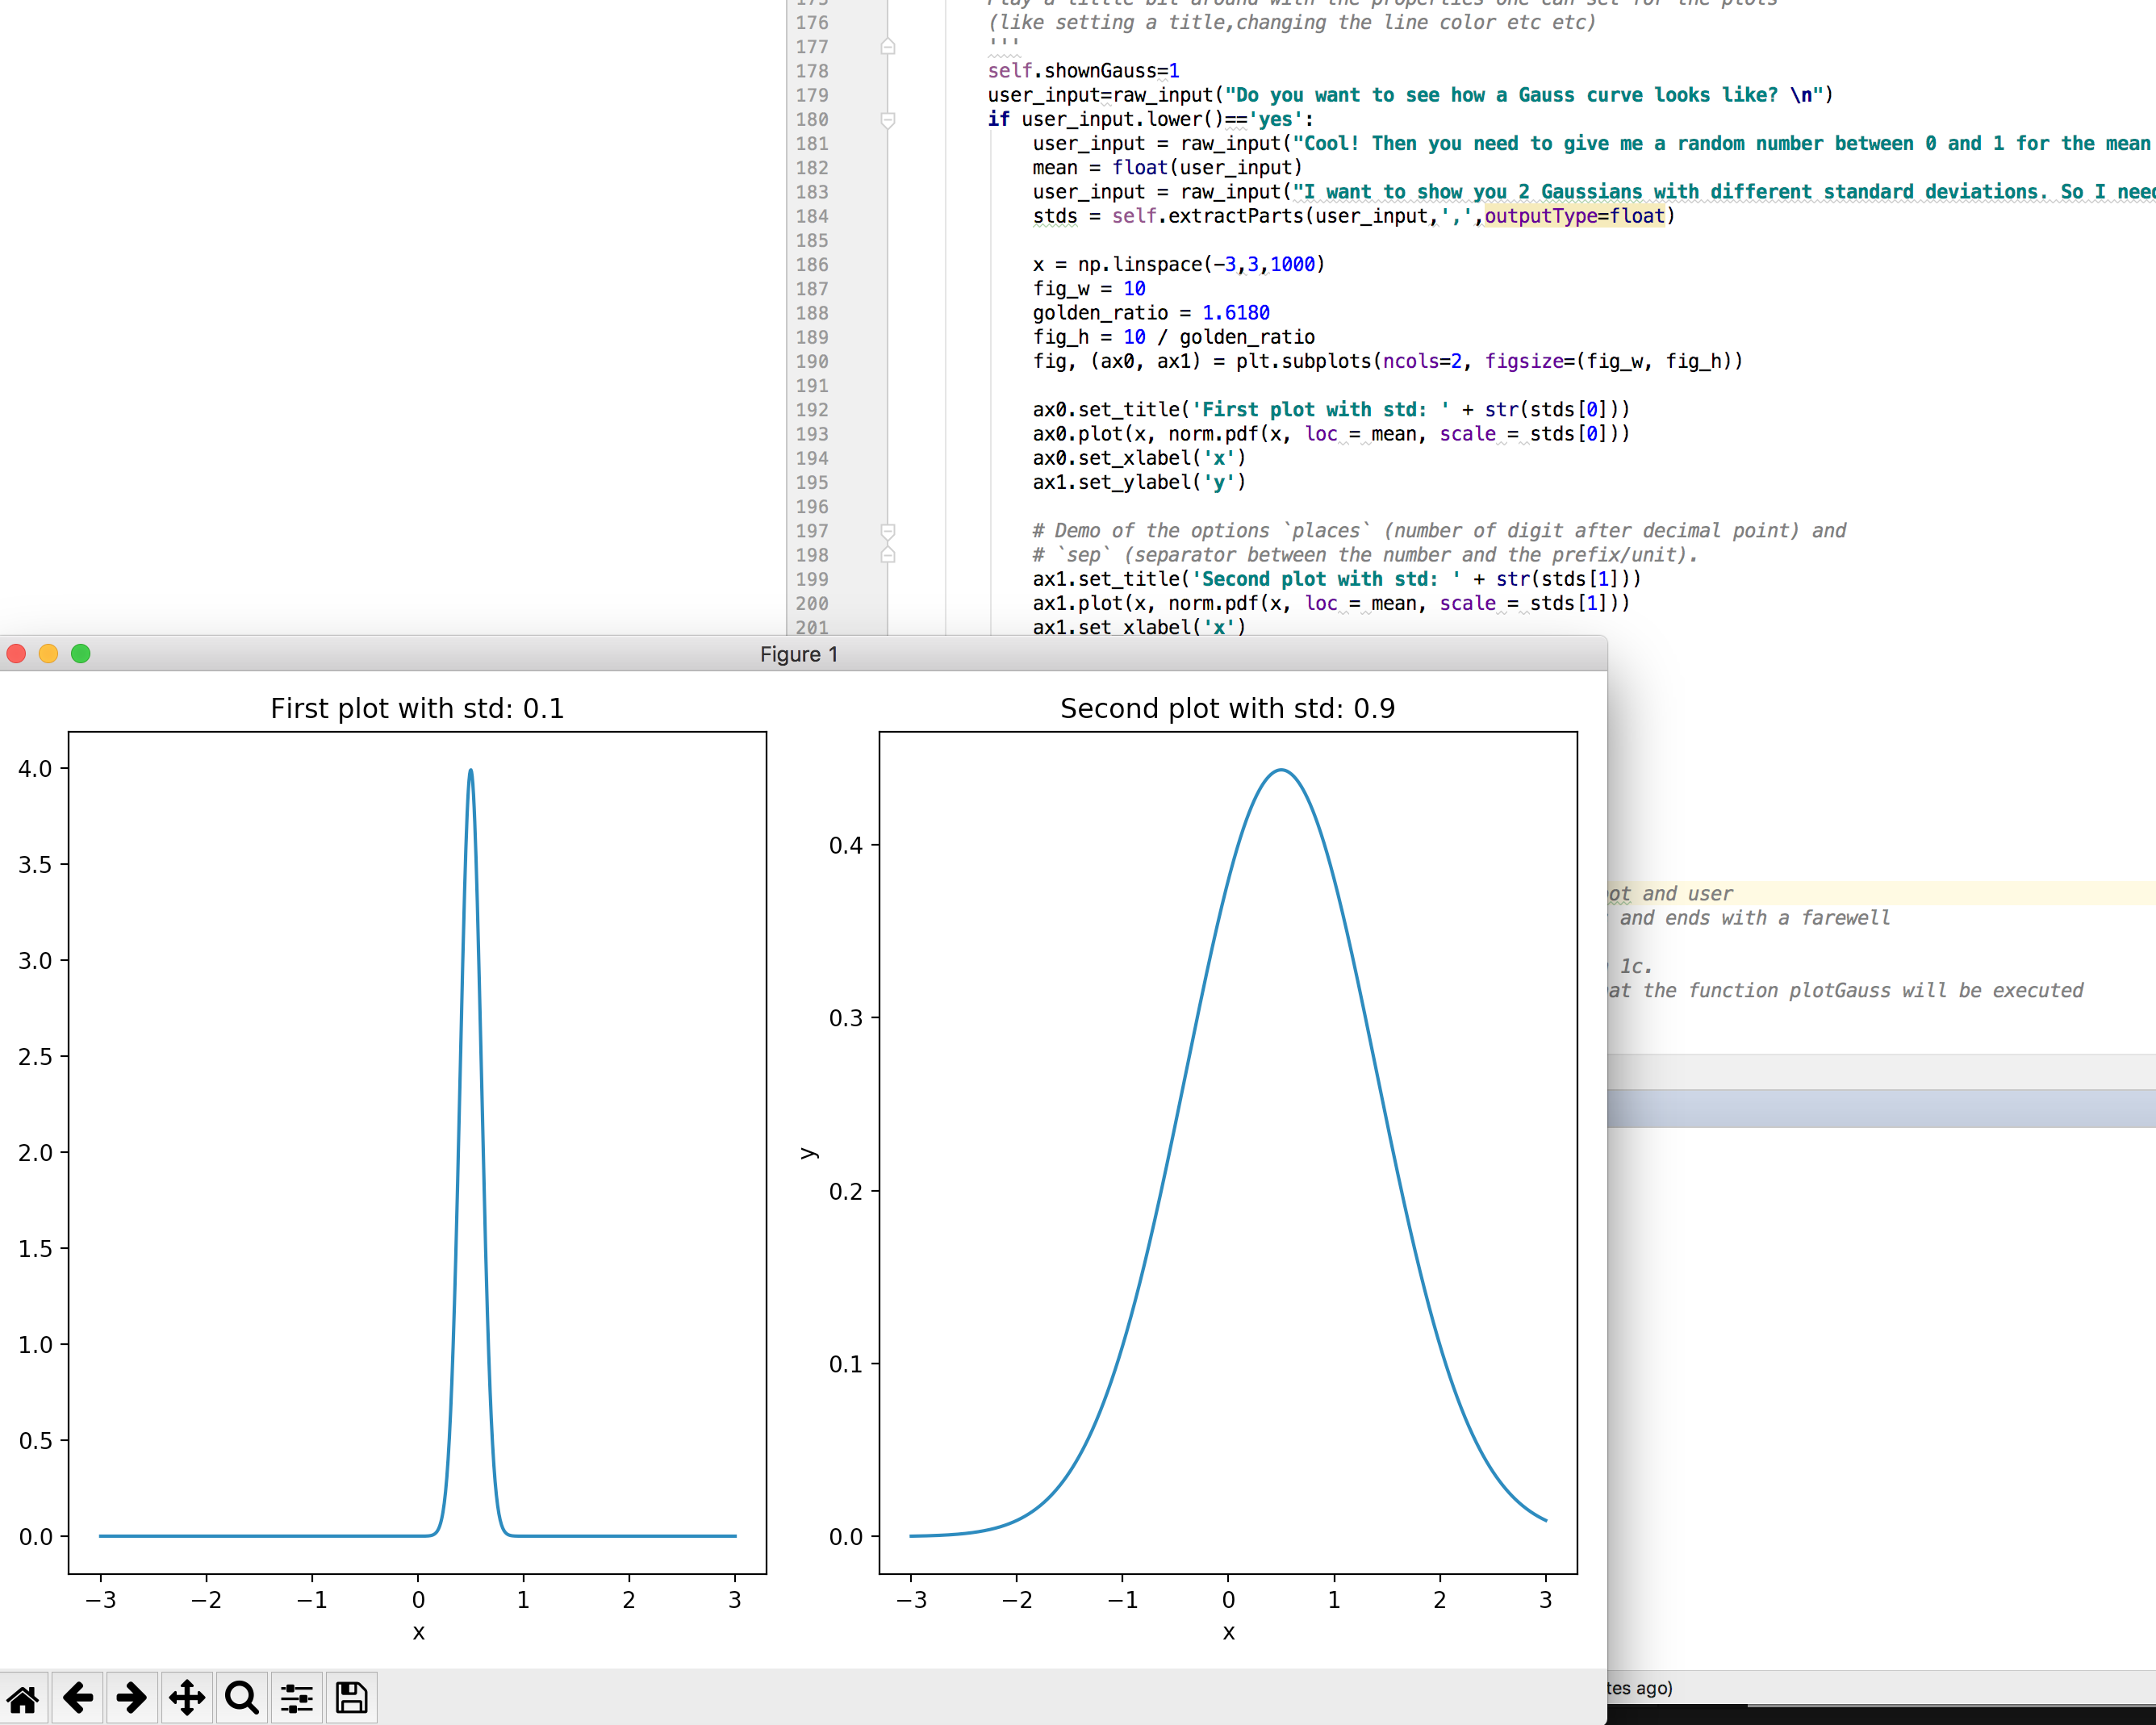
\includegraphics[width=.8\textwidth]{figures/gauss.png}
	% \caption{$jkl$ }
	\label{gauss1}
\end{figure}

\section*{Exercise 2}
(a) \textit{PEAS} is the abbreviation for Performance Measure, Environment, Actuators, Sensors.
\paragraph{Performance Measure} in the present case would be a fluent, human understandable, helpful and fast bot.
\paragraph{Environment} is the application where the bot is being used. This could be in a Facebook chat, an audio \textit{chat}bot or via email.
\paragraph{Actuators} language output, via text on a screen in a chat or via audio.
\paragraph{Sensors} are text inputs via chat, console or voice recognition software.\vspace{20pt} \\
(b) The environment is most probably fully observable (i.e. no loss of information on technical side); not deterministic because not only the bot can influence the next state of environment (human interaction); the environment is most probably static because a well performing bot should be fast (orders of ms).
The environment is not discrete, since a great amount of possible inputs are possible; probably single-agent.\\
(c) Many business sites on facebook offer chatbots. Mostly they ask easy questions which are answerable with yes / no or with a number (for example budget).
One example is SnapTravel.
Another funny example is \url{http://thebot.de/about_brain.html} which allows for interactive and open conversation.\\
(d) Our example from question 1 is a simple reflex agent, since the bot has some intelligence to determine the current state (i.e. is the current state an open question or not).
However condition-action-rules are table-lookups or very generic answers.



\newpage
\section{Appendix: Python Source Code}
Changed code to python3.
\lstinputlisting[language=Python]{chatbot.py}


\end{document}
